\documentclass{standalone}

\usepackage{tikz}
\usepackage{bm}
\usepackage{amssymb}

\usetikzlibrary{patterns}
\usetikzlibrary{arrows.meta}

\usetikzlibrary{decorations.pathreplacing, decorations.markings}
\tikzset{
    midarrow/.style={
        decoration={markings, mark=at position 0.5 with {\arrow{Latex}}},
        postaction={decorate}
    }
}

\begin{document}
	
	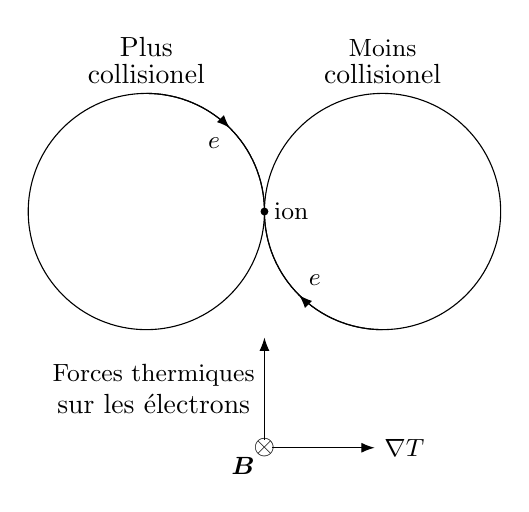
\begin{tikzpicture}
	
		\def\radius{1.5}
	
		\draw (-\radius, 0) circle [ radius=\radius ];
		\draw[ midarrow ] (-\radius, \radius) arc[start angle=90, end angle=0, radius=\radius] node[ midway, anchor=north east ] {\small \( e \)};
		\node[ anchor=south ] at (-\radius, \radius) {\shortstack{Plus\\ collisionel}};
		
		\draw (\radius, 0) circle [ radius=\radius ];
		\draw[ midarrow ] (\radius, -\radius) arc[start angle=270, end angle=180, radius=\radius] node[ midway, anchor=south west ] {\small \( e \)};
		\node[ anchor=south ] at (\radius, \radius) {\shortstack{\small Moins\\ collisionel}};
		
		\fill (0, 0) circle [ radius = 0.05 ] node[ anchor= west ] {\small ion};
		
	\def\xorig{0}
	\def\yorig{-\radius-1.5}
	\def\length{1.4}
	\def\rsymb{0.1}		
		
		\draw[ -{Latex} ] (\xorig, \yorig+\rsymb) -- (\xorig, \yorig+\length) node[ midway, anchor=east ] {\shortstack{\small Forces thermiques\\ sur les électrons}};
		
		\draw[ -{Latex} ] (\xorig+\rsymb, \yorig) -- (\xorig+\length, \yorig) node[ anchor=west ] {\small \( \nabla T \)};
		
		\draw (\xorig, \yorig) -- (\xorig, \yorig) node[ anchor=north east ] {\small \( \bm{B} \)};
		\node at (\xorig, \yorig) {\( \otimes \)};
		
	
	\end{tikzpicture}
	
\end{document}